
% \renewcommand{\cleardoublepage}{}
% \renewcommand{\clearpage}{}

%% ============================================================
%% ================= CHAPTER: Introduction ====================
%% ============================================================

\chapter{Introduction}
\label{ch:intro} 

\pagenumbering{arabic}
\setcounter{page}{1} % Start numbering from zero because command
                     % 'chapter*' does page break

Introducing the subject, the motivation behind it, methods used to investigate the problem, results found with implementing the methods and testing them.

Methods proposed in this thesis are tested in a real e-commerce website using Google Optimize to create A/B test where the A variant is the control, and the B is always the new proposed method. 

 The possible motivation for this is to identify better search engine configurations. 
\todo{Can motivation be a picture?}

Figure\ref{fig:base_conv_compare} shows that there is already an increase in conversion rate when comparing the sessions where a customer has performed a search versus the sessions where a search was not performed. 
In this thesis, the purpose is to try increase the conversion rate of the sessions where a customer performs a search operation. 
The thesis also proposes more detailed metrics to track the performance of the search results other than just the conversion rate.

\begin{figure}[h]
    \centering
    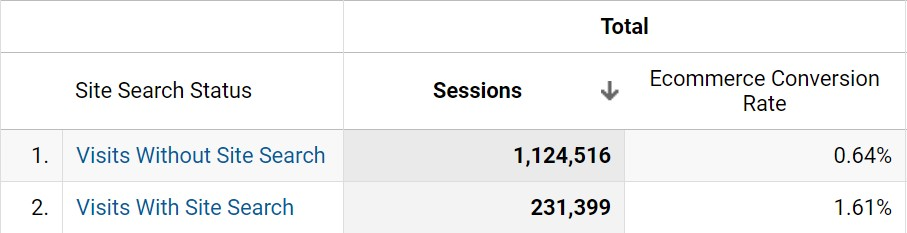
\includegraphics[width=1.0\textwidth]{img/ecom-conv-search-vs-nosearch-05_01-19_01.jpg}
    \caption{Conversion rate between the sessions with and without search from 05.01.2020 to 19.01.2020.}
    \label{fig:base_conv_compare}
\end{figure}



%% ============================================================
%% ================= CHAPTER: Background=======================
%% ============================================================

\chapter{Background}
\label{ch:background}

Background information will consist of a simplified introduction to search engines and 
how most e-commerce websites utilize them. 

\todo{list for this chapter}.
The placement of these sections might change.
\begin{enumerate}
    \item Remember to define the e-commerce conversion rate. Might be included in the \ref{ch:analysis} section.
    
    \item Remember to define the relevancy of a search result. This definition is included in section \ref{sec:relevancy} as a subsection of the search engines.

    \item What is a search engine? 
    General information about what is a search engine. 
    This section might be combined with the subsections if necessary.
    
    \begin{itemize}
        \item Introduction of a web search engine. Reference to the paper that first introduced Google \cite{googleInit}. 
        The article contains all the necessary information to introduce the basics of a web search engine.
    
        \item What is a product search engine, and how the current solution utilizes one? 
        How it traditionally differs from the web search engine?
        
    \end{itemize}

    \item Elasticsearch \cite{elasticIntro, relevantSearch} is the search engine that will be used in the testing and implementation, 
    as it is the one currently used by the organization.
    Should this be a separate chapter altogether?? I might need quite a lot of details for this chapter to make sense.
    
    \item The test setup will be implemented with Google Optimize \cite{optimizeAbout}. 
    Trying to find a better reference for this, but all the necessary information might be in the manual.
    
    \item The evaluation of the tests is done with resources provided with Google Optimize and Google Analytics \cite{optimizeAbout, analyticsAbout}. 
    Introduce the platforms and how the tests can be evaluated there.
    
\end{enumerate}

%% ==========================================================
\section{E-commerce conversion rate}
The conversion rate is an important metric in e-commerce. 
It tells what proportion of customers who visited a website resulted in conversion. 
There might be different definitions of what is a conversion in e-commerce; 
it can be, for example, a product has been added to cart, or a customer has completed a purchase
The reason why there can be multiple different types of conversions depends on the situation what is measured.
In the context of this thesis, the conversion rate is defined as what proportion of the traffic has resulted in a completed purchase.

\todo{}
\begin{itemize}

    \item There might be other conversion metrics defined in the evaluation of the relevancy of the search results...
    
    \item Add references and a lot of text.
    
\end{itemize}


%% ==========================================================
\section{What is a search engine?}
There are multiple different types of search engines. However, most people the think that a search engine is a tool that is used to find websites conveniently.



\subsection{Web search engine}
A traditional search engine is used on the web a lot and the most significant search engines are some of the most visited sites in the world \cite{alexa}.
Google is currently the leading search engine in the world and has grown and expanded ever since founded in 1998 \cite{googleInit}.



\subsection{Product search engine}
While the product search engine is based on a traditional web search engine, the functionalities and usage are different. 
What is the product search engine and how the product search differs from Google, for example?



\subsection{Relevancy of a search results}
\label{sec:relevancy}
Definition for relevancy according to \citeauthor{relevantSearch}: \cite{relevantSearch}

\begin{displayquote}
Relevance is the practice of improving search results for users by satisfying their information needs in the context of a particular user experience, 
while balancing how ranking impacts our business’s needs.
\end{displayquote}

\todo{The book also proposes the how the relevancy can be evaluated etc...}



%% ==========================================================
\section{Elasticsearch}
Elasticsearch is a distributed search and analysis engine. 
It provides document storage, which in this case, is utilized as storing the information about the products on the website. 
Elasticsearch provides many tools introduced in this section. \cite{elasticIntro}




%% ==========================================================
\section{Testing the implementation}
Testing is done with a redirect test, also known as A/B/n test, which is a randomized test where a website or part of a website is split into two or more variants. 
The traffic for the website is then redirected into the different variants at random. \cite{optimizeAbout}




%% ==========================================================
\section{Analyzing the results}
\label{ch:analysis}
The tool used to analyze the results of the proposed methods is Google Analytics.  
The tool provides a possibility to do a very detailed analysis based on the A/B/n test variants. 
\cite{analyticsAbout}

Google Optimize also provides analytical tools to evaluate the results of the tests done with it, 
but it uses Google Analytics to calculate everything \cite{optimizeAbout}. 

\todo{}
While some of the figures in the thesis are from Optimize platform, they are based on the data in Google Analytics.




%% =========================================================
%% ================= CHAPTER: Methods=======================
%% =========================================================
\chapter{Methods}
\label{ch:methods}

\citeauthor{relevantSearch} proposed multiple different solutions on how the relevancy of the search results could be improved.
Elasticsearch provides multiple build-in tools which are defined individually when necessary. \cite{relevantSearch}

\todo{} 
Also define what index and search times mean.

%% ==========================================================
\section{Text analysis tools}
\label{sec:textAnalysisTools}
In this section, necessary text analysis tools are introduced, 
firstly the purpose and usage of the tools and secondly how the individual tools work and how they are utilized in the thesis.

The tools used in this thesis are mostly the different kinds of analyzers, tokenizers, and filters 
used to analyze the text fields of the documents that are relevant to the search. 
Elasticsearch provides a wide range of different build-in analysis tools, 
but there is a possibility to also define custom tools, for example, customer analyzers, 
which could be in the text field analysis. \cite{elasticIntro}

\todo{} 
Subsections will include more detailed information about the individual analysis tools used in the thesis.
Includes the tools used in both index time and search time.

%% ==========================================================
\subsection{Analyzers}
A analyzer is a text analysis process that converts the input text into tokens or terms in index time, 
which are used in the inverted index in the search time. 
\cite{elasticIntro}

%% ==========================================================
\subsection{Tokenizers}
A tokenizer is used to break up a stream of characters into a stream of individual tokens in index time. 
In search time, tokens are used to match the query and evaluate the relevancy of the match.
\cite{elasticIntro}


%% ==========================================================
\subsection{Token filters}
Token filters are used to filter the results of a tokenizer. 
It can be used to modify the individual tokens or, for example, to filter out the unnecessary tokens.
\cite{elasticIntro}



%% ==========================================================
\section{Search analysis}

There are multiple tools provided to analyze the input queries. This section is for introducing those.
\cite{relevantSearch}

\todo{There will be more subsections in this chapter.} Just what I came up with 

\subsection{Query}
How the query is handled and composed in Elasticsearch. 
How the queries are matched to the fields in the inverted index, that have been analyzed by the tools mentioned in section \ref{sec:textAnalysisTools}.

\subsection{Ranking algorithms}
The other part of searching for anything is to rank the search results.
The ranking of the search results might be the most important thing when it comes to searching.

\todo{}
There is already a ranking system in place in the current solution so tell something about it and propose a better way of doing things.


%% ============================================================
%% ================= CHAPTER: Testing =========================
%% ============================================================
\chapter{Testing the methods}
\label{ch:testmethods}
The placement of this section is not defined yet, for now, its own section.
Section \ref{ch:methods} defined a lot of different tools, so the purpose of this section is to define the different test cases and define the tools used in them.

This section will be determined when I have had a chance to read the whole book from \citeauthor{relevantSearch} \cite{relevantSearch} and 
evaluated other ways to implement different solutions that could be useful to test.


%% ============================================================
%% ================= CHAPTER: Results =========================
%% ============================================================
\chapter{Results}

The comparison of the results of the methods proposed.


\begin{itemize}
    \item \citeauthor{relevantSearch} \cite{relevantSearch} have proposed how the relevancy of the search results could be analyzed. 
    
    \item The current plan is to generate heat maps of the different solutions if those are seen as useful.

    \item At least the calculation of how different the specified metrics used in the evaluation are different compared to the control.
    Google Analytics provides a lot of metrics that can be used here.     
\end{itemize}

So most likely, there will be quite a few pictures in this section and information about the pictures. \cite{analyticsAbout}


%% ============================================================
%% ================= CHAPTER: Conclusions =====================
%% ============================================================
\chapter{Conclusions}
What was done in this thesis, and what conclusions could we draw from it.



%% ============================================================
\section{Future work}
What this thesis did not include, but a future implementation could.

\begin{itemize}
    \item At least the search personalization. 
    This might need to be introduced at some point but is not included in this theses.
\end{itemize}



%% ============================================================
\section{Problems?}
Mention possible problems, if there were any, here, which might have affected the results.


